\documentclass[12pt]{article}
\usepackage{graphicx}

\usepackage{hyperref}
\hypersetup{
  colorlinks=true,
  linkcolor=black,
  filecolor=magenta,      
  urlcolor=cyan,
}
\begin{document}

\title{Coding Standards Document}
\maketitle
\center{\textbf{Team Name:} Binary Ninjaz\\}
\center{\textbf{System Name:} Harvest\\}

\includegraphics[scale=0.3]{harvestIcon.png}
\center{\textbf{Client Name:} Barry Christie\\ }
\center{\textbf{Team Members:\\} 
Teboho Mokoena (u14415888)\\
Sizo Duma (u15245579)\\
Letanyan Delon Arumugam (u14228123)\\
John Ojo (u15096794)\\
Kevin Reid (u15008739)\\
Shaun Yates (u16007493)\\ }
  \newpage
  
  \tableofcontents
  \newpage

  \section{Detailed System Design}
  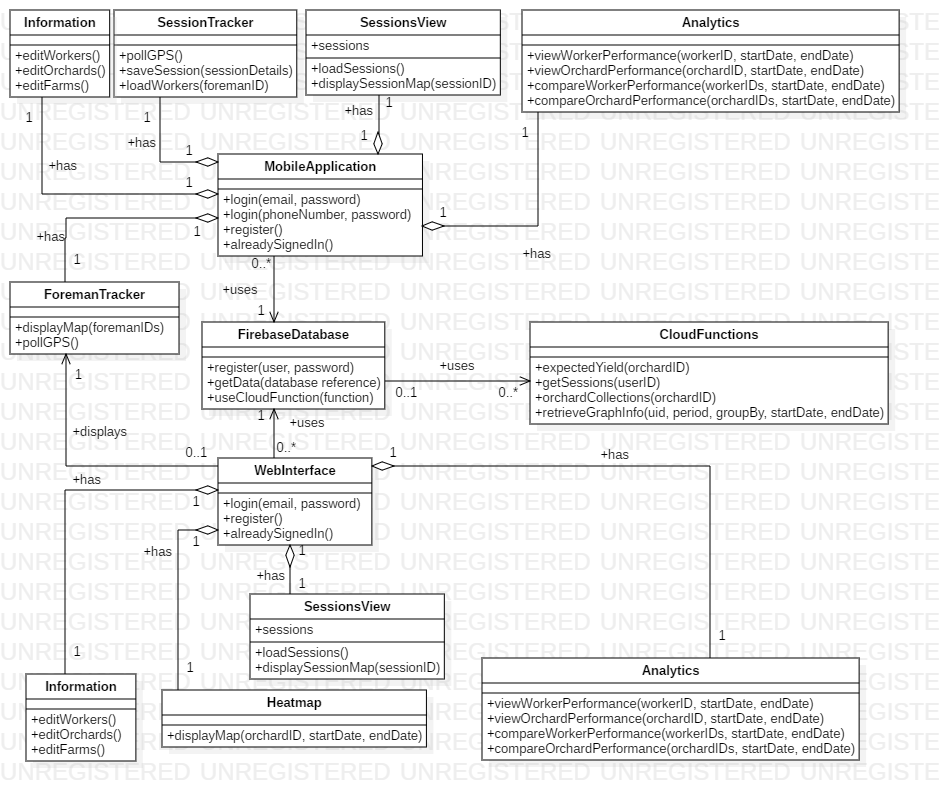
\includegraphics[width=1.2\linewidth]{UMLClassDiag.png}
  \newpage
  
  \section{Coding Conventions}
  \flushleft
  The project and design we've undertaken means that we will need to use multiple languages and IDE's to complete the project. As such we have decided that the best common practice and standards of each language shall be the standard that is used for that respective language/environment.
  \subsection{HTML/CSS}
  The HTML and CSS standards we shall follow will be the ones of \href{https://google.github.io/styleguide/htmlcssguide.html}{Google's HTML/CSS style guide}
  
  \subsection{JavaScript}
  For JavaScript we will be using \href{https://google.github.io/styleguide/jsguide.html}{Google's JavaScript style guide}.
  
  \subsection{Java}
  Similarly we will use \href{https://google.github.io/styleguide/javaguide.html}{Google's Java style guide}.
  \subsection{Swift}
  For Swift we will use \href{https://swift.org/documentation/api-design-guidelines/}{Apple design guidelines}.
  
  \center\section{File Structure}
  \includegraphics[width=1.2\linewidth]{FileStructure.png}
  \flushleft\subsection{Branching}
  
  An example structure is shown above, showing that \texttt{master} is never worked on directly. Each subsystem has its own respective branch, and these branches branch off \texttt{Developer}, and in turn any changes done to a branch would then branch off that specific branch. A \texttt{Developer} branch is used, to act in much the same way as \texttt{master}, but as a proxy, so that before merging that branch to master, the entire system can be reviewed there before a more solid commitment is made.
  \subsection{Naming}
  \flushleft
  A branch shall never contain an individuals name, rather it must be informative as to what the intention of the branch is whilst also remaining short. An example of a  name that would be deemed unacceptable is \texttt{Joe}; another would be \texttt{JoeWebsiteChanges}, where the name contains a member name, and gives very little information as to what is going on in the branch. Bad, but barely acceptable names are \texttt{WebsiteChanges}, or \texttt{WebsiteExperimentation}. Ideal names are as follows: in the case of a branch where the website is ultimately being assembled, by merging other branches into it, and the only modifications taking place are to structure the files, or a quick fix, such as changing the colour of a button, \texttt{Website}; in the case that a new homepage is created for the website, where the homepage is created, and merged into \texttt{Website} on completion, \texttt{Website-Homepage}. Finally, if a user wants to propose a change to the \texttt{Website-Homepage} branch, where he wants to change the colour of a button, but the user has not been assigned, or is not the primary benefactor to \texttt{Website-Homepage}, he creates a new \texttt{Website-Homepage-ButtonColourChange} branch. Notice that in the ideal examples it is possible to track down the source of a branch, to understand exactly what it's purpose is.
  
  \center\section{Code Review Process}
  \flushleft
All code reviewing is done on GitHub, and occurs every time there are changes done to code, or if new code has been implemented. Currently, pre-commit reviews are utilized and although it is a slower process compared to post-commit reviews, it always for more people to be aware of changes to the code and could possibly lead to better implementation as more eyes usually means more ideas. \newline
After changes have been made on the branch, the creator, who wants to merge, will then make a pull request on GitHub, and announce the request on Slack. After which it shall become the responsibility of the entire team, but more importantly that of the original branch maintainer to analyze and comment on the changes. The exact location of the discussion is trivial, however GitHub provides a better, and more concrete platform for this discussion to take place, where inline comments can be made. After a sufficient amount of time and discussion has passed, either the branch maintainer (if it is a minor change), or the entire team (if it is to master, or a major change) shall decide to merge or not.

  
\end{document}